\documentclass[graybox]{svmult}
\usepackage[hang]{footmisc}
\setlength{\footnotemargin}{0pt}
\usepackage{footmisc,multicol, graphicx,makeidx,courier,helvet}
\usepackage[latin1]{inputenc}
\usepackage{amssymb,amsmath,amsthm} 
%\usepackage{mathptmx}
\usepackage{amsfonts}
\usepackage{graphicx}
% choose options for [] as required from the list
% in the Reference Guide

\usepackage{mathptmx}       % selects Times Roman as basic font
\usepackage{helvet}         % selects Helvetica as sans-serif font
\usepackage{courier}        % selects Courier as typewriter font
\usepackage{type1cm}        % activate if the above 3 fonts are
                            % not available on your system
%
\usepackage{makeidx}         % allows index generation
\usepackage{graphicx}        % standard LaTeX graphics tool
                             % when including figure files
\usepackage{multicol}        % used for the two-column index
%\usepackage[bottom]{footmisc}% places footnotes at page bottom
% see the list of further useful packages
% in the Reference Guide

\makeindex             % used for the subject index
                       % please use the style svind.ist with
                       % your makeindex program
\begin{document}
\def\s{\sigma}


\title*{An informational approach to the Network Disease Hypothesis in resting
state fMRI}
\author{Jaime Gomez-Ramirez, Yujie Li, Qiong Wu, Xiaoyu Tang, Jinglong Wu}
\institute{ \at  Biomedical Engineering Laboratory, Okayama University,  Japan
\\ Autonomous Systems Laboratory, Universidad Polit�cnica de Madrid, Spain \\
 \email{jd.gomez@upm.es}}
 
\maketitle

\abstract{Here
we combine graph and information theory based approaches to understand network
robustness in resting state-fMRI (R-fMRI). We calculate how the network
robustness is affected upon the removal of nodes in the functional
connectivity network in resting state for both young and elder subjects.
We find that \ldots
predictor of aging?
Then, we study the stochastic process defined by a random walk on the
functional connectivity graph, to provide information theoretic measures such
as the entropy rate of the stationary Markov chain. We find that the entropy
rate of the functional connectivity network modeled as a Markov chain explains
why the removal of some nodes increases the efficiency of the informational
flow shown in the graph based approach. 
We argue that the discovery of network
based biomarkers for neurodegenerative conditions will rely on the combination
of both graph theoretic and informational approaches in R-fMRI.
}

\keywords{resting state fMRI, network degeneration hypothesis, Markov chain,
relative entropy}


\section{Introduction}
%Relevance of RS 

It has been suggested that fluctuations in the BOLD signal measured
in humans in resting state, represent the neuronal activity baseline and shape
spatially consistent patterns \cite{Raichle:2005}, \cite{Fransson:2006}. These
slow fluctuations in the BOLD signal found in resting subjects, are highly
coherent within either structural or functional networks in the human brain. Therefore,
exploring these fluctuations could lead to a better understanding of the
brain's intrinsic or spontaneous neural activity.
Functional correlation based on the synchrony of low-frequency blood flow
fluctuations in resting state, have been identified in the sensorimotor
\cite{kokkonen_preoperative_2009}, visual \cite{damoiseaux_consistent_2006},
language \cite{hampson_detection_2002}, auditory
\cite{hunter_neural_2006}, dorsal and ventral attention
\cite{fox_spontaneous_2006} and the frontoparietal control system
\cite{vincent_evidence_2008}.
The systematic study of those patterns using correlation
analysis techniques has identified a number of resting state networks, which
are functionally relevant networks found in subjects in the absence of either
goal directed-task or external stimuli.

%Seed based versus ICA 
The visual identification of the
overall connectivity patters in resting state functional magnetic resonance
imaging (R-fMRI), has been assessed using either model-based and model-free
approaches. In the former, statistical parametric maps of brain activation are
built upon voxel-wise analysis location. %references HERE
This approach has been successful in
the identification of motor networks, but it shows important limitations when
the seed voxel cannot be easily identified. For example, in brain areas with
unclear boundaries i.e., cognitive networks involved for instance, in language
or memory. Independent Component Analysis (ICA), on the other hand, is a
model-free approach that allows separating resting fluctuations from other
signal variations, resulting on a collection of spatial maps, one for each
independent component, that represent functionally relevant networks in the
brain. 
%Bad sentence, improve style
While ICA has the advantage over model-free methods that it is unbiased,
(that is, it does not need to posit a specific temporal model of correlation
between ROIs), the functional relevance of the different components is,
however, computed relative to their resemblance to a number of networks based
on criteria that are not easily formalized.

%Review on GT methods 
More recently, researchers using graph-theory based methods have been able to
not only visualize brain networks, but to quantify their topological properties. Large-scale anatomical
connectivity analysis in the mammalian brain, shows that brain topology is
neither random nor regular. Instead, small world
architectures \cite{Watts:1998} -highly clustered nodes connected thorough
relatively short paths- have been identified in brain networks. 
%\cite{Vaessen:2010}.
Small world networks are not solely
structural, functional networks with a small world organization have been
identified in the mammal brain \cite{Bassett:2006}. In addition to
this, disruptions in the small world organization can give clues about normal
development and pathological conditions. For example, Supekar and colleagues
\cite{Supekar:2008} have shown that the deterioration of small world
properties such as the lowering of the cluster coefficient, affect local
network connectivity, which in turn may work as a network biomarker for
Alzheimer's disease. Abnormalities in small-worldness may also have a
significant positive correlation in, for example, schizophrenia
\cite{liu_disrupted_2008} and epilepsy \cite{liao_altered_2010}. While
network-based studies have been successful in delineating generic network properties, such as
path length or clustering, additional work is needed in order to come to grips
with the internal working of the systems underlying the network. 

%review on Info. Theory methods
REVIEW INFO THEORY in resting state functional connectivity 


 %%%%%%%%%%%%%%%% 
In this paper we investigate the effects of aging in resting state
functional connectivity nertworks using  using a methodology that combines
graph and information theoretic tools. ESTO FUERA, FOCUS ON RW
In section \ref{mat-methods} the methodology followed in the data acquisition,
data preprocessing, anatomical parcellation and brain network reconstruction
in two groups -24 young and 19 elder individuals- is presented. 
Then, we systematically study network
robustness -functional network invariance under perturbation- is affected upon
the removal of nodes in the functional connectivity network in resting state
for both young and elder subjects. We provide a ranking of nodes that
quantifies the impact of their obliteration using a network efficiency measure
based on \cite{latora_efficient_2001} that quantifies how the network
efficiency in transmitting information deteriorates once a node is removed from the network.
This is described in the results section
\ref{results}. The paper concludes with a discussion section \ref{discussion}.
PLUS RW. STUDY ROBISTNESS first by removal of nodes and its edges and rank
using Melchiori measure and then study robustness in network dynamics.

%it is sketched a new theoretical framework to investigate network robustness
%and how it is affected by internal perturbations such as aging. 

%!* (LI) Now, refer to both Young and Elder 
\section{Materials and Methods}
\label{mat-methods}
%Materials Experimental (Li)
\subsection{Subjects}
Twenty-three healthy male volunteers (ages 21-32; mean 22.7) took part in the
fMRI experiment. All subjects had normal or corrected-to-normal vision. The
study was approved by the ethics committee of Okayama University, and written
informed consent was obtained before the study. 
\subsection{Data acquisition}
 All subjects were imaged using a 1.5 T Philips scanner vision whole-body MRI
 system (Okayama University Hospital, Okayama, Japan), which was equipped with
 a head coil. Functional MR images were acquired during rest when subjects were
 instructed to keep their eyes closed and not to think of anything in
 particular. The imaging area consisted of 32 functional gradient-echo planar
 imaging (EPI) axial slices (voxel size=3x3x4 mm3, TR=3000 ms, TE=50 ms,
 FA=90�, 64x64 matrix) that were used to obtain T2*-weighted fMRI images in the
 axial plane. We obtained 176 functional volumes and excluded the first 4 scans
 from analysis. Before the EPI scan, a T1-weighted 3D magnetization-prepared
 rapid acquisition gradient echo (MP-RAGE) sequence was acquired (TR=2300 ms,
 TE=2.98 ms, TI=900 ms, voxel size=1x1x1 mm3).

\subsection{Data preprocessing} 
Data were preprocessed using Statistical Parametric Mapping software SPM8
\footnote{http://www.fil.ion.ucl.ac.uk/spm/} and REST v1.7
\footnote{http://restfmri.net/forum/index.php}. To correct for differences in
slice acquisition time, all images were synchronized to the middle slice.
Subsequently, images were spatially realigned to the first volume due to head
motion. None of the subjects had head movements exceeding 2.5 mm on any axis or
rotations greater than 2.5�. After the correction,  the imaging data were
normalized to the Montreal Neurological Institute (MNI) EPI template supplied
with SPM8 (resampled to 2x2x2 mm3 voxels) \footnote{http://imaging.mrc-cbu.cam.ac.uk/imaging/Templates}. In order to avoid
artificially introducing local spatial correlation, the normalized images were
not smoothed. Finally, the resulting data were temporally band-pass filtered
(0.01-0.08 Hz) to reduce the effects of low-frequency drifts and high-frequency
physiological noises \cite{jiao_granger_2011}.

\subsection{Anatomical parcellation} 
Before whole brain parcellation, several sources of spurious variance including
the estimated head motion parameters, the global brain signal and the average
time series in the cerebrospinal fluid and white matter regions were removed
from the data through linear regression \cite{REF}. Then, the fMRI data
were parcellated into 90 regions using an automated anatomical labeling template \cite{REF}.
For each subject, the mean time series of each region was obtained by simply
averaging the time series of all voxels within that region.

\subsection{Brain network construction} 
To measure the functional connectivity among regions, we calculated the Pearson
correlation coefficients between any possible pair of regional time series, and
then obtained a temporal correlation matrix $(90x90)$ for each subject. We
applied Fisher's r-to-z transformation to improve the normality of the
correlation matrix. Then, two-tailed one-sample t-tests were performed for all
the possible 4005 i.e., $\frac{90x89}{2}$ pairwise correlations across subjects
to examine whether each inter-regional correlation significantly differed from
zero. 

\begin{figure}[!h]
\begin{center}
\centerline{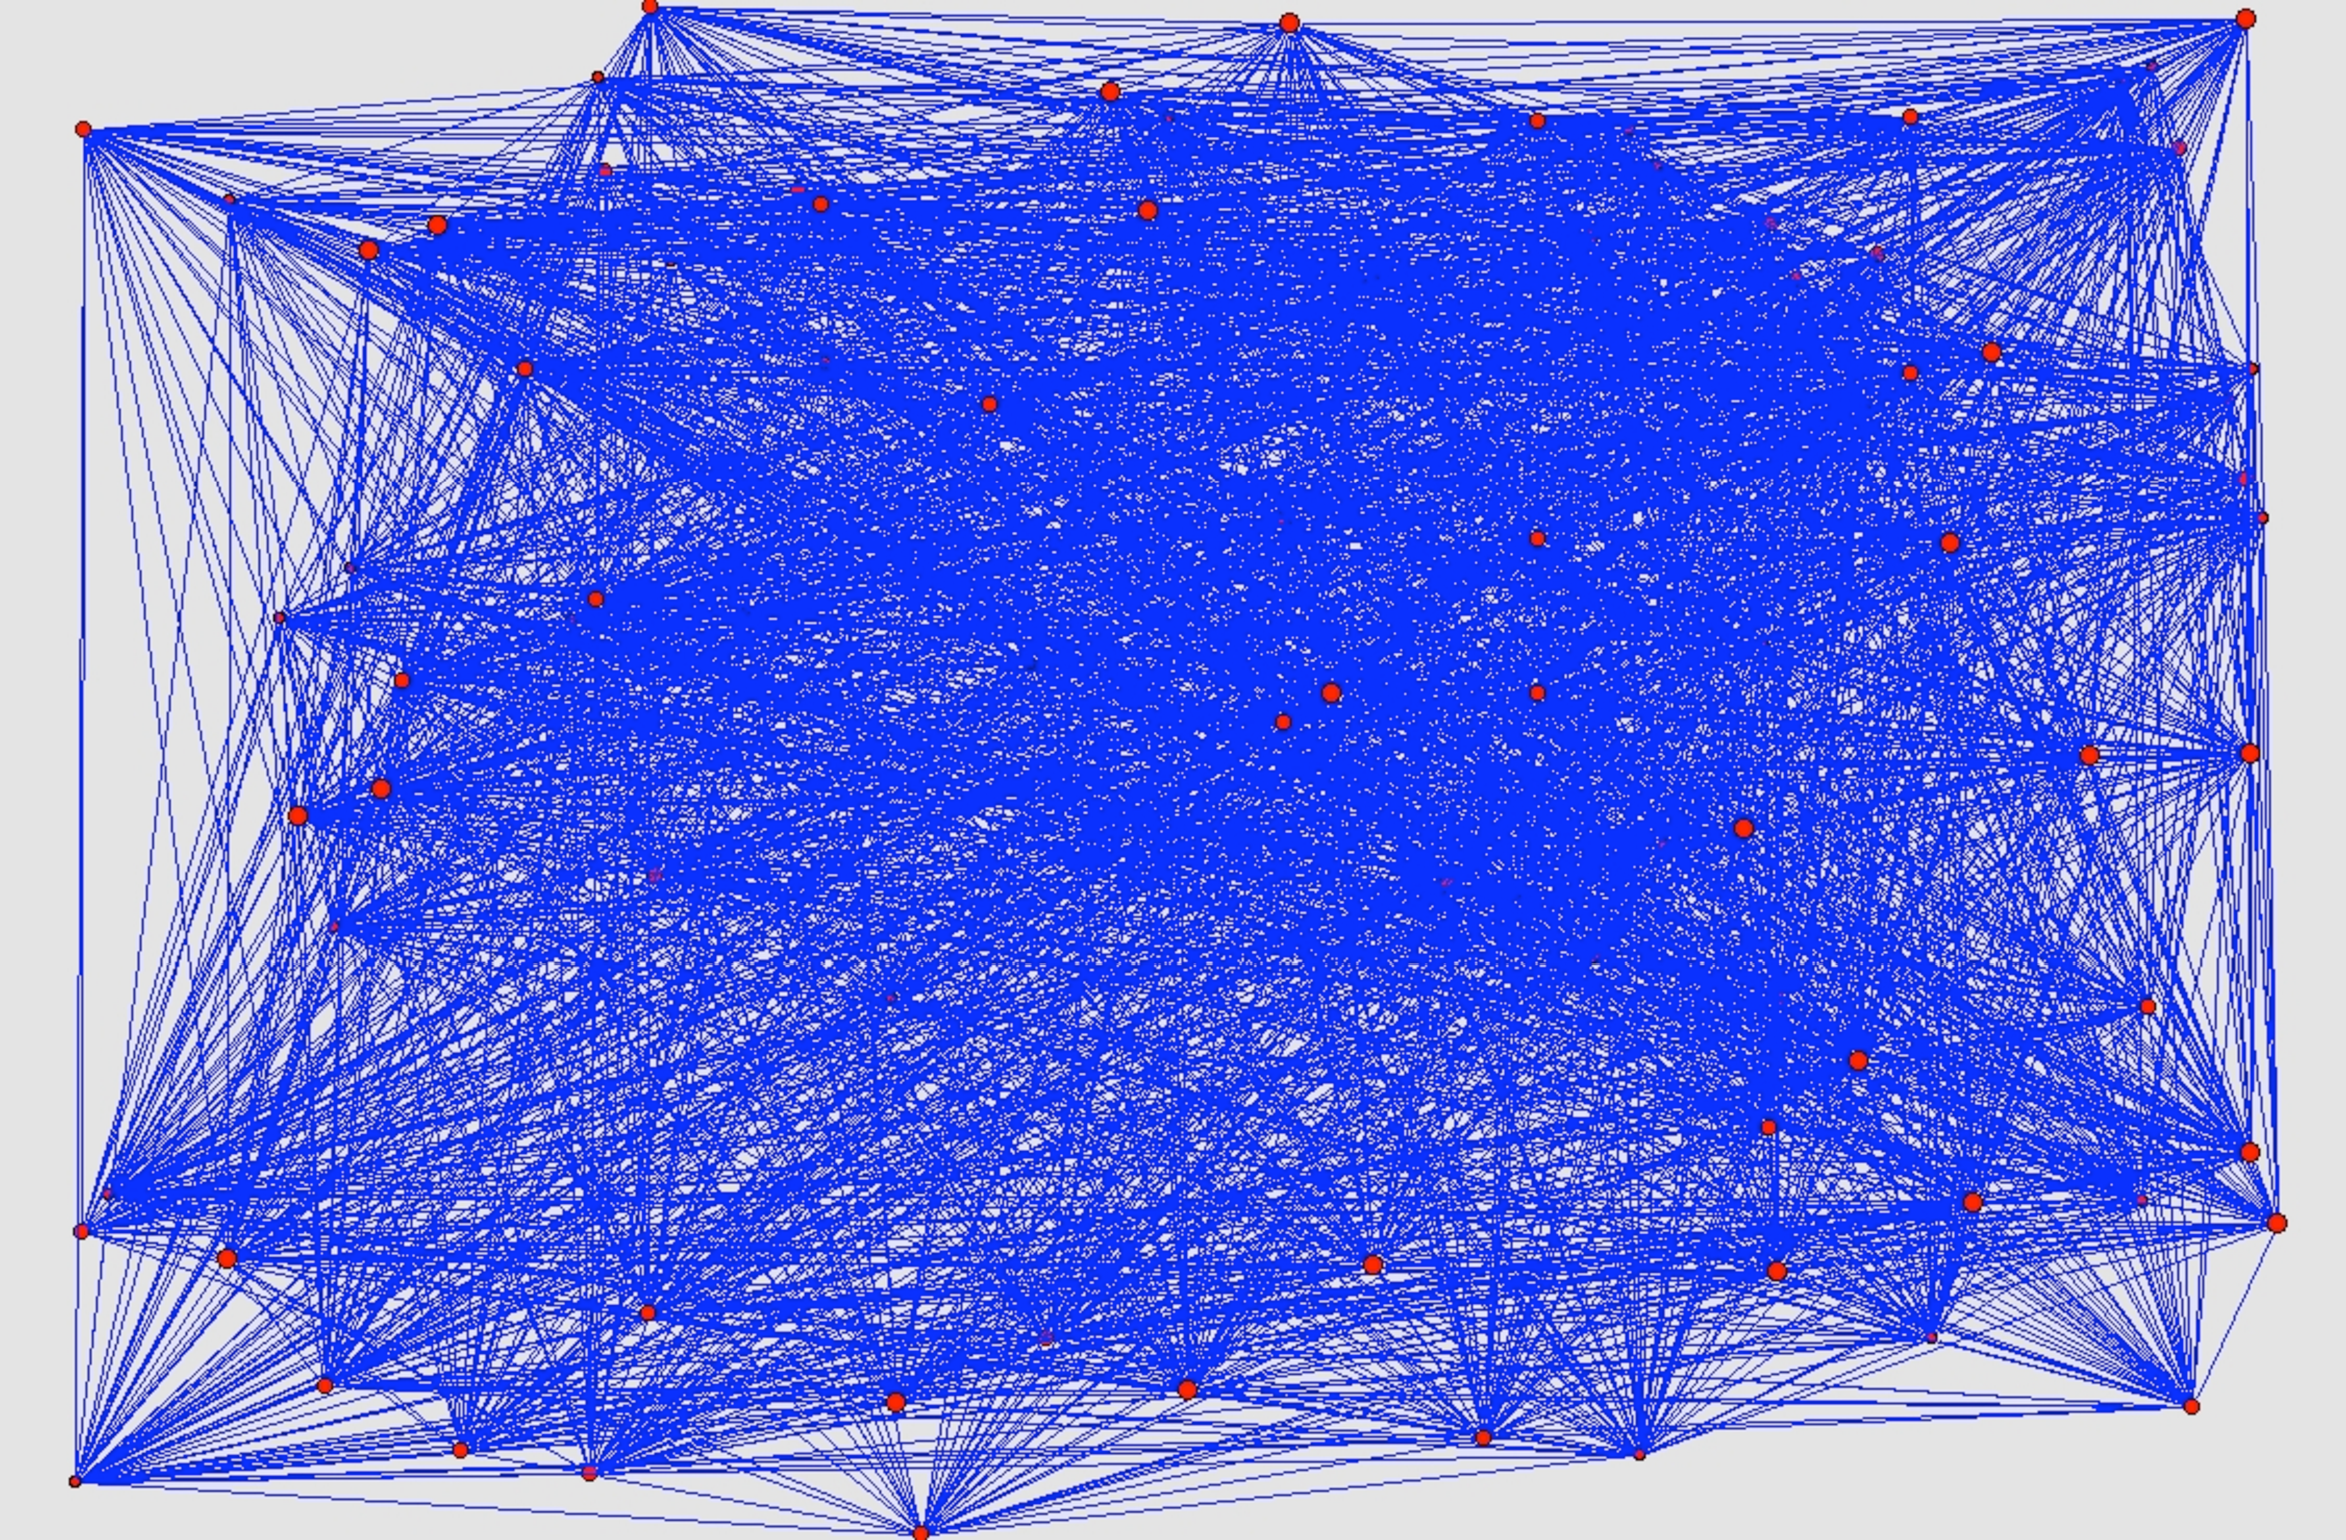
\includegraphics [scale=0.4]  {figures/Pajek9090.pdf}}
\caption{Graphic representation of the functional connectivity
among regions based on the temporal correlation matrix of the twenty-three
healthy controls, using Pajek software \cite{batagelj_pajek_2004}}
\label{Fig:Pajek}
\end{center}
\end{figure} 

A Bonferroni-corrected significance level of $P<0.001$ was
further used to threshold the correlation matrix into an adjacency matrix whose
element was 1 if there was significant correlation between the two brain
regions and 0 otherwise. Finally, an undirected binary graph was acquired in
which nodes represent brain regions and edges represent links between regions.
The study of the connectivity distribution of the resulting adjacency matrix is
provided in the Appendix \ref{appendix}.

% GT
\subsection{Graph theoretic analysis}
Until the recent advent of graph theoretic methods in R-fMRI, the focus was
put on the identification of anatomically separated regions that show a
high level of functional correlation during rest. 
The tools we use to model a system may also convey an ontological
version of it, that is to say, the system under study is seen through the
lens of a specific approach that necessarily shapes the observability domain. 
Thus, the identification of different subnetworks during rest can be seen as a
 by-product of the techniques used, for example identification component
 analysis (ICA) or clustering. 
Graph theory provides a
theoretical framework to investigate the overall architecture of the brain.
The use of graph theoretic techniques to model brain networks has shifted the 
emphasis from the identification of local subnetworks -default mode network,
primary sensory motor network etc.- to the quantitative study of the topological
and informational characteristics of large-scale brain networks.
Graph theory-based approaches model the brain as
 a complex network in which nodes represent brain regions of interest and the
 edges connecting nodes represent relationship between nodes e.g., functional
 connectivity. 
 
 The graph-based network provides a geometric representation to
 visualize brain connectivity patterns and an analytic toolbox to
 quantitatively characterize the overall topological organization.   
 %adv
Graph-based techniques have proliferated in the last years providing new
insights into the structure function relationship in the healthy brain, and
in aging and neuropathological disorders \cite{fair_functional_2009}, 
\cite{wang_graph-based_2010}, \cite{he_graph_2010}. Prove of the utility of this
approach is that notable proponents of a modularist vision of brain
connectivity to understand cognition, such as Gazzaniga
\cite{gazzaniga_new_1999} (see \cite{Fuster:2000} for an early critic of the
modularist approach by Fuster who anticipates a shift toward a networks) has
now embraced the complex brain networks approach to understand the interplay
between structure and function in brain systems \cite{bassett_understanding_2011}.
%disv motifs

\subsubsection{Network robustness, efficiency and node vulnerability}
\label{ss:nrobeffvul}
%Distance related measures (Network Efficiency and Network Vulnerability)
A critical aspect is to understand network robustness, that is, functional
network invariance under perturbation. In essence, robustness measures the
capacity of the network to perform the same function before and after a
perturbation. Perturbations are events, internal or external, that elicit a
change in the network configuration, as for example in, to obliterate a node or
a change in the connectivity between nodes. 
Thus, for a given network  $G(N,E)$ with an adjacency matrix $A$, a perturbation
$\delta$ (e.g., the removal of a set of nodes $M$ from $N$) transforms $A$ into
a new adjacency matrix $A'$. Thus, the initial graph $G(N,E)$ is transformed
into a new post perturbation graph $G(N-M,E-E(M))$, where $E-E(M)$ is the set
of edges that do not connect any of the deleted nodes in $M$. 
Now we want to calculate the robustness of the network to the perturbation
$\delta$. Robustness is here studied as a loss in the efficiency. Thus, the
robustness measure, $\mathcal{R}$ for a network $G$ is defined as the relative performance
retained or efficiency loss under a network insult i.e., a perturbation $\delta$, 
that transforms the initial network $G$ into $G^{\delta}$.
\begin{equation}
\mathcal{R^{\delta}}(G)= \frac {\Sigma(G^{\delta)}} {\Sigma(G)}
\label{eq:rob}
\end{equation}
Thus, from equation \ref{eq:rob}, a network $G$ is considered to be robust (to
a perturbation $\delta$) if the network performance or efficiency $\Sigma(G)$
stays close to the original value after a perturbation, ideally $\mathcal{R^{\delta}}=1$. 
 %The dual of
 %robustness in vulnerability. Therefore, Vulnerability $\mathcal{V}$ is here
 %used as the complementary of robustness, therefore $\mathcal{V^{\delta}}+
 %\mathcal{R^{\delta}}=1$
 
Now, we need to provide the formal definition of network efficiency. The
efficiency of a network $G$, $\Sigma(G)$, is a network centrality
measure that quantifies the network's reliability in transmitting information, once a
node or a set of nodes have being removed. The network efficiency can be 
calculated using the Latora and Marchiori measure
\cite{latora_efficient_2001}. Accordingly, the efficiency in the communication
between any two nodes  in a graph G is equal to the inverse of the shortest path that
connects them or $\varepsilon_{ij}= \frac{1} {d_{ij}}$. The
efficiency of the graph is calculated as the average of the efficiency between
any two nodes $\varepsilon_{ij}$ 
\begin{equation}
\Sigma(G)=\frac{\sum_{i \neq j \in G} \varepsilon_{ij}} {N(N-1)}
=\frac{1}{N(N-1)}\frac{1}{\sum_{i \neq j \in G} d_{ij}}
\label{eq:latm}
\end{equation}
where $N$ is the number of nodes and $d_{ij}$ is the
shortest path length (the geodesic distance) between nodes $i$ and $j$. 
According to equation \ref{eq:latm}, the quantity $\Sigma(G)$ is defined in the
range $[0,1]$ and measures the mean flow-tare of information over G. Thus, a 
graph G with $\Sigma(G)=l$ is more efficient than a graph $H$ with $\Sigma(H)=m$,
if and only if $l > m$.
Note that when there is no path that connects the nodes i and j, $d_{ij}=
\infty$, and the efficiency in the communication of the two nodes is zero,
$\varepsilon_{ij}=0$.


%%%%%%%%%%%%%%%%%%%%%%%%%%%%%%%%%%%%%
%%%%%%%%%%%%%%%%%%%%%%%%%%%%%%%%%%%%%

The global network efficiency is 0.3678 for young subjects and 0.1144 for elder
subjects. Thus, young subjects connectivity network is three times more
efficient in terms of the shortest path distance between any two nodes.
%Use ``graphshortestpath'' to calculate shortest path problem in 
%from http://www.mathworks.es/es/help/bioinfo/network-analysis-and-visualization.html

We can, in addition to robustness and efficiency of G calculate the information
centrality C of any node i in the network G as the variation in the
network efficiency caused by the removal of the edges incident in i. The
centrality of a node i $C_i$ is calculated as the difference between the
efficiency of the original graph G with N nodes and E edges , G(N,E), and the
efficiency of the resulting graph $G_i$ with N nodes and $E-k_i$ edges. Thus, the centrality of a node is a
normalized measure of the loss in network efficiency caused by the isolation of
a node in G.
\begin{equation}
C_i=\frac {\Sigma(G(N,E)) - \Sigma(G(N,E-k_i)) } {\Sigma(G(N,E))} 
\label{eq:centr}
\end{equation}
By the same token, the information centrality of a set of nodes $S$ can be
calculated as normalized measure of the loss in network efficiency caused by the isolation of
a set of nodes S in G.
\begin{equation}
C_S=\frac {\Sigma(G(N,E)) - \Sigma(G(N,E-k_S)) } {\Sigma(G(N,E))} 
\label{eq:centrS}
\end{equation}




In Table \ref{Table:BA} (see Excel file) is shown the information
centrality for each of the AAL regions.

%LI: Do you think is a good idea to remove entire networks , e.g., DMN (AAL 23,
%24, 25, 26) rather than single nodes as I did ?

%'' The investigators showed that
%focal lesions located in the precuneus, medial anterior
%cingulate cortex, temporo-parietal junction, or superior
%frontal cortex produced widespread and substantial
%changes in functional connectivity with intrahemispheric
%and contralateral regions. Conversely, lesions to the
%visual or motor cortices had restricted effects on global
%connectivity.49  Alstott J, Breakspear M, Hagmann P, Cammoun L, Sporns O.
%Modeling the impact of lesions in the human brain.
%PLoS Comput Biol 2009; 5: e1000408.

%%%%%%%%%%%%%%%%%%%%%%%%%%%%%%%%%%%%%
%%%%%%%%%%%%%%%%%%%%%%%%%%%%%%%%%%%%%
\subsection{Information theoretic analysis on Markov chains}
The undirected binary graph depicted in Figure \ref{Fig:Pajek} is the geometric
characterisation of the adjacency matrix $A$, in which $a_{ij}=1$ if AAL region
$i$ and AAL region $j$ show a significant correlation, and $a_{ij}=0$ otherwise.
We transform the binary adjacency matrix $A$ into a weighted adjacency matrix
$T$, where $T_{ij}=\frac {a_{ij}} {\sum_{j} {a_{ij}}}$. Thus, the new graph has
the same number of nodes and the  weight connecting any two nodes is  $T_{ij}$.
Note that $T_{ij} = 0$ if nodes are not connected, symmetry is preserved 
$T_{ij}= T_{ji}$.

Now, let us consider a random walk -a particle moving from node to node- on the
weighted undirected graph $T$. A random walk $\{X_1 \ldots X_n\}$ is defined as
the list of nodes visited by the particle. The probability that the particle
moves from i to j is given by $T_{ij}$. This stochastic process defines a
Markov chain because the probability that the particle moves from state
$n$ to state $n+1$ is independent of the previous states, that is,
$P(X_{n+1}=x_{n+1}|X_{n}=x_{n})= P(X_{n+1}=x_{n+1}|X_{n}=x_{n},X_{n-1}=x_{n-1}, \ldots ,X_{1}=x_{1})$.
%%Check WSD toolbox

The stationary distribution of the random walk on the undirected graph is 
$\mu=\{\frac {k_1} {2E}, \frac {k_2} {2E}, \ldots , \frac {k_N} {2E}\}$, where
$k_i$ is the connectivity degree of node i and E is the total number of links
contained in the graph. It ought to be noted that the
stationary distribution does not depend on the number of nodes, but only on the total
number of links E, and the weight (or the number) of links connecting each
node. Thus, the stationary distribution holds the local property that it is not altered by
changes in the weights of non neighbors nodes, while keeping the total weight
of the graph constant.
 
The entropy rate of a stochastic process represents the rate at
which the entropy of a sequence e.g., a random walk, grows with n. Formally, for
the stochastic process $\mathcal{X}=\{X_1, \ldots , X_n\}$ the
entropy rate is given by
\begin{equation}
H(\mathcal{X})= \lim_{n \to \infty}\frac{1}{n} H(X_1, X_2, \ldots , X_n)
\end{equation}
For a stationary Markov chain, the entropy rate is  
\begin{equation}
H(\mathcal{X})= \lim_{n \to \infty} H(X_n |�X_{n-1}, \ldots , X_1)=  \lim_{n \to
\infty} H(X_n  | X_{n-1}) =  \lim_{n \to
\infty} H(X_2  | X_{1})
\end{equation}
%The entropy rate is computed with the stationary distribution of the Markov
%chain $\mu$ and the transition matrix $T$. Then
%\begin{equation}
%H(\mathcal{X})= - \sum_{ij} \mu_i T_{ij}\log  T_{ij} 
%\end{equation}

We define a Markov process for both the young subjects and the elder ones
with their transition matrix given by $T_{ij}^{y}$ and $T_{ij}^{e}$ respectively
\begin{equation}
\begin{array}{l}
\displaystyle  T_{ij}^{y}=\frac {A_{ij}^{y}} {\sum_{j} {A_{ij}^{y}}} \\
\displaystyle T_{ij}^{e}=\frac {A_{ij}^{e}} {\sum_{j} {A_{ij}^{e}}} 
\end{array}
\end{equation}
where $A_{ij}^{y}$ and  $A_{ij}^{e}$ are the binary adjacency matrix of the
young and the elder subjects. Thus, the entropy rate is
\begin{equation}
\begin{array}{l}
\displaystyle H(\mathcal{X}^{y}) = - \sum_{ij} \mu^{y}_{i}  T_{ij}^{y} \log 
T_{ij}^{y} \\
 \displaystyle  H(\mathcal{X}^{e}) = - \sum_{ij} \mu^{e}_{i}  T_{ij}^{e} \log 
T_{ij}^{e}
\end{array}
\label{eq:enrate}
 \end{equation}

We calculate the entropy rate for the resulting Markov process after
having removed all the edges incident to a node i $\mathcal{X}_{i}$. Thus, the
transition matrix $T'$ for the Markov process $\mathcal{X}_{i}$ is such that
$T'=T$ except for both the column and row i which are all 0,
$T'_{i,}=T'_{,i}=0$. The relative entropy of this new stochastic process
$\mathcal{X}_{i}$ is:

\begin{equation}
\begin{array}{l}
\displaystyle H(\mathcal{X}_{i}) = - \sum_{k,j, k \neq i} \mu_{k} 
T'_{kj} \log T'_{kj}
\end{array}
\label{eq:tijenrate}
 \end{equation}

By the same token, the entropy rate when the edges incident to any of the nodes
of the components of the set of nodes S are removed is 
\begin{equation}
\begin{array}{l}
\displaystyle H(\mathcal{X}_{S}) = - \sum_{k,j, k \neq S} \mu_{k} 
T'_{kj} \log T'_{kj}
\end{array}
\label{eq:Senrate}
 \end{equation}

Analogously to the information centrality $C_i$ defined in \ref{eq:centr}, 
we calculate the normalized value $D_i$ defined as the difference between the
entropy rate of the original Markov process, $\mathcal{X}$, and the resulting
process of deleting the edges incident in i, $\mathcal{X}_{i}$. 
\begin{equation}
\begin{array}{l}
\displaystyle D_i = \frac{H(\mathcal{X})-H(\mathcal{X}_{i})}{H(\mathcal{X})}
\end{array}
\label{eq:Diffenrate}
 \end{equation}
By the same token, when the resulting Markov process is given by the removal
of the edges incident in any of the nodes in a set S $\mathcal{X}_{S}$ we have
\begin{equation}
\begin{array}{l}
\displaystyle D_S = \frac{H(\mathcal{X})-H(\mathcal{X}_S)}{H(\mathcal{X})}
\end{array}
\label{eq:SDiffenrate}
 \end{equation}

%%%% CALCULATION

%!* Biased vs unbiased 
%To calculate the entropy rate we follow \cite{gomez-gardenes_entropy_2008} in
%which the Markv process is a biased random walk with a probability for the
%walker to move from node i to node j proportional to the power$\alpha$ of the
%destination node degree $k_j$ . The transition
%probability matrix os this kinfd of biased random walk is given by the
%expression:
%\begin{equation}
%\begin{array}{l}
%\displaystyle T_{ij} = \frac {A_{ij}k_{j}^\alpha}�{\sum_{j}A_{ij}k_{j}^\alpha}
%\end{array}
%\label{enrategeneral}
 %\end{equation}
%Note that the parameter $\alpha$ allows to tune the bias. Thus, when $\alpha
%>0$ the walker tends to visit neighbors with high degree and when $\alpha <0$
%the walker tends to visit more ofter neighbors that are poorly connected.
%Here, for simplicity, we assume that the random walk is unbiased, so $\alpha =
%0$ and the transitivity matrix is
%\begin{equation}
%\begin{array}{l}
%\displaystyle T_{ij} = \frac {A_{ij}}�{\sum_{j}A_{ij}}
%\end{array}
%\label{erateunbiased}
 %\end{equation}
%!* call function [h alpha] =entropy_rate(A,alpha) from WSD toolbox


\section{Results}
\label{results}

We have analyzed the functional connectivity in resting state of both young and
elder individuals. The nodes representing the ninety brain regions based on the
AAL parcelation have been ranked in terms of their impact in terms of network
robustness upon removal. Interestingly we find that in both elder and young
groups the removal of certain nodes does not necessarily triggers a
decrease in network robustness, the obliteration of certain nodes may also 
produces a positive impact in the network function, increasing the  network
robustness  when the node is removed.
We study network robustness based on the new network efficiency/performance
 measure (equation \ref{eq:latm}) to investigate the network
 functionality when a set of nodes are obliterated. 
The results show that in young subjects, the nodes with a positive impact
are \ldots TO DO LI/JAIME compared with elder subjects \ldots TO DO LI/JAIME.

In the second part we use information-theoretic measures to study the impact of
the removal of nodes in the network. First, we model the network flows in terms
of a stationary Markov chain which describes how a particle walks randomly from
node to node, in both the young and elder functional connectivity graph. The
probability transition matrix is derived from the binary adjacency matrix using
the local property of connectivity degree.
The entropy rate of a
random walk on a graph in which a node or group of nodes has been removed is
calculated.

The results show that in young subjects, after he removal of the nodes with
a positive impact the entropy rate is $> <?$ TO DO JAIME than in the case of
elder subjects.




%!* Future work
%DELETE NETWORKS OF INTEREST RATHER THAN SINGLE NODES 
%For example, DMN is commonly considered to consist of medial prefrontal cortex
%(AAL 23, 24, 25, 26), posterior cingulate cortex/precuneus (AAL 35, 36/67 68)
%and bilateral inferior parietal lobule (AAL 61, 62). In the case of elder
%individuals, COMPLETE. RELATE RESULTS  with the literature on RSNs . 

%What can
%we say about this vulnerability ranking and the robustness of RSNs and the NDH

%!* relate this results with the litterature on RSNs . What can we say about
% this vulnerability ranking and the robustness of RSNs and the NDH?

   

\section{Discussion}
\label{discussion}

\section{Appendix}
\label{dse:appe}
Imformation is a concept too broad to be captured in a sigle definition,
however, for any probability distribution we have the entropy, which is a
quantity that agree with the intuitive notion we may have about information.
Entropy can be extended to the mutual information which is the amount of
entropy that one random variable contains about another. Entropy is then a
special case of the M becuase, entropy is the self information of a random
variable, H(X)=MI(X,X). And MI is a special case of the relative entropy or
distance between two probability distributions.

     H is special case of MI is a special case of relativeH or KL
     
     Notation: The  netropy is of a random variable, H(X) but we can also write
     H(p) where p is the pmf of the r.v. X. Note that p(x)=Pr(X=x), for all x
     in the support of X.
     
     A stochastic process is a indexed sequence of random variables and it can
     be described as the joint probability mass function.
     A stoch process is stationary if the joint distribution is invariant with
     time shifts.
     A distribution on the states at time n = 
      Markov is en example of a stoch. process with dependence, each
     r.v dependes respoec to shifts in the time index.
     on the one preceding it and is conditionayy independent of all the other
     preceding r.v. 
\bibliographystyle{ieeetr}
%\bibliography{~/Eclipse/workspace/BiblioTex/bibliojgr}
\bibliography{bibliojgr}

\end{document}